% \documentclass[aspectratio=169,notes]{beamer}
\documentclass[aspectratio=169]{beamer}
\usetheme[faculty=phil]{fibeamer}
\usepackage{polyglossia}
\setmainlanguage{english} %% main locale instead of `english`, you
%% can typeset the presentation in either Czech or Slovak,
%% respectively.
\setotherlanguages{russian} %% The additional keys allow
%%
%%   \begin{otherlanguage}{czech}   ... \end{otherlanguage}
%%   \begin{otherlanguage}{slovak}  ... \end{otherlanguage}
%%
%% These macros specify information about the presentation
\title[Theoretical Mechanics]{Week HW 3, COMPLEX} %% that will be typeset on the
\subtitle{ Complex motion \\
\ \\ \
         } %% title page.
\author{Oleg Bulichev}
%% These additional packages are used within the document:
\usepackage{ragged2e}  % `\justifying` text
\usepackage{booktabs}  % Tables
\usepackage{tabularx}
\usepackage{tikz}      % Diagrams
\usetikzlibrary{calc, shapes, backgrounds}
\usepackage{amsmath, amssymb}
\usepackage{url}       % `\url`s
\usepackage{listings}  % Code listings
% \usepackage{subfigure}
\usepackage{floatrow}
\usepackage{subcaption}
\usepackage{mathtools}
\usepackage{todonotes}
\usepackage{fontspec}
\usepackage{multicol}
\usepackage{pdfpages}
\usepackage{wrapfig}
\usepackage{animate}
\usepackage{booktabs}
\usepackage{multirow}
% \usepackage{graphicx}
\usepackage{colortbl}

\graphicspath{{resources/}}
\frenchspacing

\setbeamertemplate{caption}[numbered]
\usetikzlibrary{graphs}

% \usepackage[backend=biber,style=ieee,autocite=footnote]{biblatex}
% \addbibresource{biblio.bib}
% \DefineBibliographyStrings{english}{%
%   bibliography = {References},}

\newcommand{\oleg}[2][] {\todo[color=red, #1] {OLEG:\\ #2}}
\newcommand{\fbckg}[1]{\usebackgroundtemplate{\includegraphics[width=\paperwidth]{#1}}}%frame background

\usepackage[framemethod=TikZ]{mdframed}
\newcommand{\dbox}[1]{
\begin{mdframed}[roundcorner=3pt, backgroundcolor=yellow, linewidth=0]
\vspace{1mm}
{#1}
\vspace{1mm}
\end{mdframed}
}

\begin{document}
\setlength{\abovedisplayskip}{0pt}
\setlength{\belowdisplayskip}{0pt}
\setlength{\abovedisplayshortskip}{0pt}
\setlength{\belowdisplayshortskip}{0pt}

\fbckg{fibeamer/figs/title_page.png}
\frame[c]{\setcounter{framenumber}{0}
    \usebeamerfont{title}%
    \usebeamercolor[fg]{title}%
    \begin{minipage}[b][6.5\baselineskip][b]{\textwidth}%
        \textcolor{black}{\raggedright\inserttitle}
    \end{minipage}
    % \vskip-1.5\baselineskip

    \usebeamerfont{subtitle}%
    \usebeamercolor[fg]{framesubtitle}%
    \begin{minipage}[b][3\baselineskip][b]{\textwidth}
        \raggedright%
        \insertsubtitle%
    \end{minipage}
    \vskip.25\baselineskip
}
%   \frame[c]{\maketitle}

\fbckg{fibeamer/figs/common.png}

\begin{frame}[t]{Task 1}
    \begin{minipage}{0.6\textwidth}
      You should find an absolute velocity and coriolis acceleration, and absolute acceleration of particle $M$ at the time $t=t_1$. 
      
      Needed variables:\\
      $OM=s_r(t)=f_3(t)=2t^3+3t$;\\
      $\phi(t)=f_2(t)=\frac{1}{24}\pi t^2$;\\
      $t_1=2,\ R=15$.
    \end{minipage}
    \begin{minipage}{0.39\textwidth}
      \vspace*{-0.5cm}
      \begin{figure}[H]
        \centering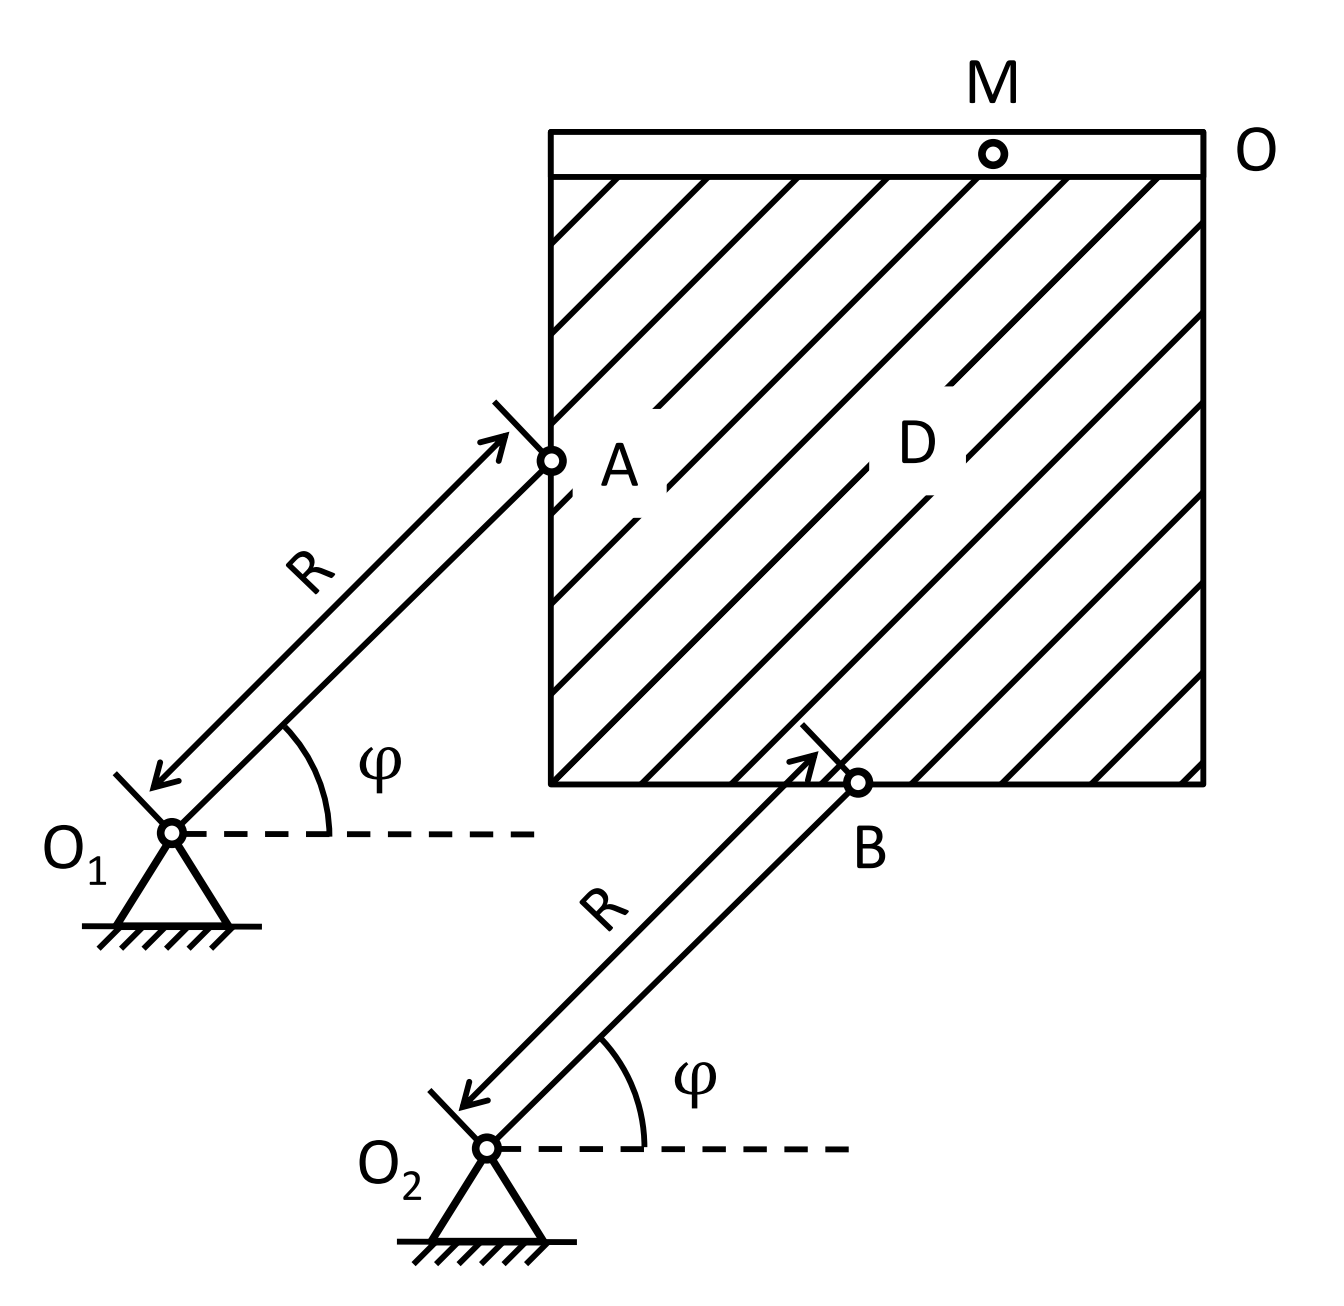
\includegraphics[height=6cm,width=1\textwidth,keepaspectratio]{HW3_1}
        \caption*{Task 1 \\ (Yablonskii (eng) K-5)}
      \end{figure}
    \end{minipage}
  \end{frame}
  
  \begin{frame}[t]{Task 2 (Coding)}
    \begin{minipage}{0.65\textwidth}
      You should find:
      \begin{enumerate}
          \item simulate this mechanism (obtain all positions);
          \item Find absolute, transport and relative velocities and accelerations for $M$;
          \item Find $t$, when $M$ reaches $O$ point;
          \item draw plots $v_{rel},\ v_{tr},\ a_{tr},\ a_{rel},\ a$ respect to time.
      \end{enumerate}
      Needed variables:\\
      $\phi_e=f_1(t)=0.2t^3+t$;\\
      $OM=s_r=f_2(t)=5\sqrt{2}(t^2+t)$;\\
      $a=60,\ \alpha = 45$.
    \end{minipage}
    \begin{minipage}{0.34\textwidth}
      \begin{figure}[H]
        \centering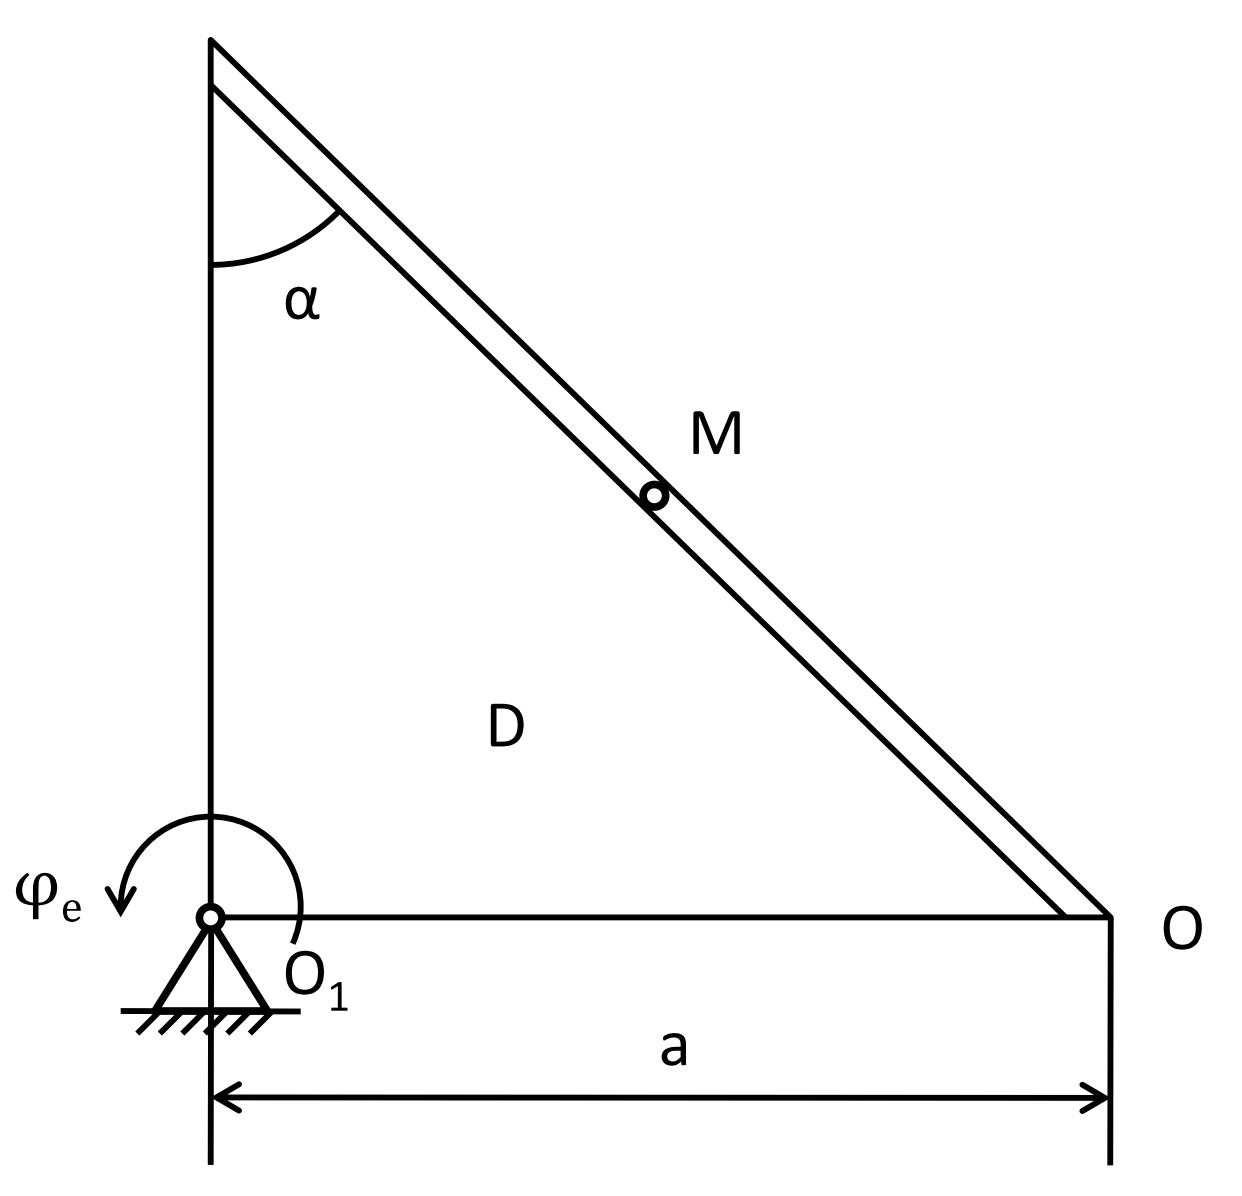
\includegraphics[height=5cm,width=0.99\textwidth,keepaspectratio]{HW3_2}
        \caption*{Task 2 \\ (Yablonskii (eng) K-6)}
      \end{figure}
    \end{minipage}
  \end{frame}

\fbckg{fibeamer/figs/last_page.png}
\frame[plain]{}
\end{document}